\documentclass[11pt]{article}

\usepackage{graphicx}
\usepackage{amsmath}
\usepackage[pdftex]{hyperref}
\usepackage[compact]{titlesec}
\usepackage{algpseudocode}
\usepackage{algorithm}
\titlespacing{\section}{0pt}{0.5cm}{*0}
\titlespacing{\subsection}{0pt}{0.3cm}{*0}
\titlespacing{\subsubsection}{0pt}{0.2cm}{*0}
\setlength{\parindent}{0cm}
\setlength{\parskip}{0.1cm}
\setlength{\parsep}{0.1cm}
\setlength{\headheight}{0cm}
\setlength{\headsep}{0cm}
\renewcommand{\baselinestretch}{1}
\renewcommand{\familydefault}{\sfdefault}
\usepackage{geometry}
\geometry{
    a4paper,
    total={210mm,297mm},
    left=25mm,
    right=25mm,
    top=20mm,
    bottom=20mm,
}
\usepackage{caption} \captionsetup[table]{skip=10pt}


\title{Text Categorisation \\\vspace{1mm} {\Large Information Retrieval Milestone II Report}}
\author{Ruifeng Xu\\ ruxu@student.ethz.ch\\}
\date{\today}

\begin{document}
\maketitle

\section{Introduction}
The goal of this text categorisation task is to predict the topics of different Reuter news documents based on their textual content.
This report briefly summarises the implementation and the performance of the three text classifiers. 
Specifically, the three classification models implemented are Naive Bayes (NB), Logistic Regression (LR) and Support Vector Machine (SVM).
The report also provides instructions on how to use them. 

\section{Implementation \& Evaluation}
Since each Reuter document in the dataset can belong to multiple topics, a one-vs-any classifier is learned for each topic.
To predict the topics of a new Reuter document, the textual content of the document is passed to each classifier, and the classifier will determine whether to give a positive (the document should be assigned the topic the classifier represents) or a negative (the document does not belong to the topic) feedback.
In the end, all responses from every classifier is grouped together to achieve the effect of multi-class classification.

\subsection{Feature Extraction}
In this project, all three classification models use the bag-of-word representation of the Reuter document as their input features.
Therefore, the first step of the experiment is to extract individual words from the corpus.
In order to achieve better feature extraction result, an external natural language processing library called Processors\footnote{https://github.com/sistanlp/processors}, which in turn is based on the Stanford CoreNLP\footnote{http://nlp.stanford.edu/software/corenlp.shtml} library, is used to tokenise and lemmatise the title and content of the Reuter document. 
Afterwards, stop words are removed based on the list provided by ranks.nl\footnote{http://www.ranks.nl/stopwords}.
Also, the topics of each document, if available, is extracted and stored.
This information is used during training phase as well as the performance evaluation phase. 
Note that the use of extra natural language processing techniques, especially lemmatisation, has lead to a longer running time of feature extraction.

\subsection{Notations}
This section formalises the notations to be used in the rest of the report.
In this project, we assume that there is a corpus $D$ consisting of various Reuter documents $d$, i.e. $d\in D$.
Each document $d$ is assigned to one or more topics.
A topic is denoted by $t$, and the set of all possible topics is denoted by $T$.
The content of each document $d$ is a bag of words.
If we denote each individual word as $w$, then a document is represented by $\{w_1, w_2, ..., w_n\}$.
The set of all unique words $w_i$'s appeared in the corpus $D$ is called the vocabulary of the corpus, denoted by $V$.


\subsection{Naive Bayes}

\subsubsection*{Learning}
For the NB classifier, we need to estimate the prior probability $P(t)$ for each topic $t\in T$, and the conditional probability $P(w|t)$ for each word $w \in V$, given that the topic under consideration is $t$.
Using the Bayes' rule and assuming conditional independence, the posterior probability $P(t|d)$, or $P(t|w_1, w_2, ..., w_n)$, where $w_i\in d$, can be calculated as

\begin{equation}
    \label{eq:nb-bayes}
    \begin{split}
        P(t|d) & = \cfrac{P(t)P(d|t)}{P(d)} \\
            & = \cfrac{P(t)P(w_1, w_2, ..., w_n|t)}{P(d)} \\
            & \propto P(t)\prod\limits_{i=1}^n P(w_i|t)
    \end{split}        
\end{equation}

To address the problem of sparsity, Laplace smoothing technique is introduced.
The following equations shows the rules to estimate the probabilities.

\begin{equation}
    \label{eq:nb-prior}
    \begin{split}
        \hat{P}(t) & = \cfrac{number\ of\ documents\ in\ D\ assigned\ to\ topic\ t}{total\ number\ of\ documents\ in\ D}
    \end{split}
\end{equation}

\begin{equation}
    \label{eq:nb-likelihoood}
    \begin{split}
        \hat{P}(w|t) & = \cfrac{1 + \sum\limits_{d\in D\ and\ t\in topics(d)} term\_frequency(w, d)}{size(V) + \sum\limits_{d\in D\ and\ t\in topics(d)} size(d)}
    \end{split}
\end{equation}


\subsubsection*{Prediction}
The NB classifier implemented in this project predicts a fixed number of topics for each document passed to it, which can be specified programmatically.

\subsubsection*{Performance}
Figure \ref{fig:nb} shows the performance of the prediction under various configurations. 
It can be seen that the best performance in terms of average F1 score is achieved when the number of topics to emit is set to $3$.
The corresponding average precision, average recall and average F1 score are $0.7374$, $0.7510$, and $0.7194$ respectively.

\begin{figure}[b]
\centering
    \centering
    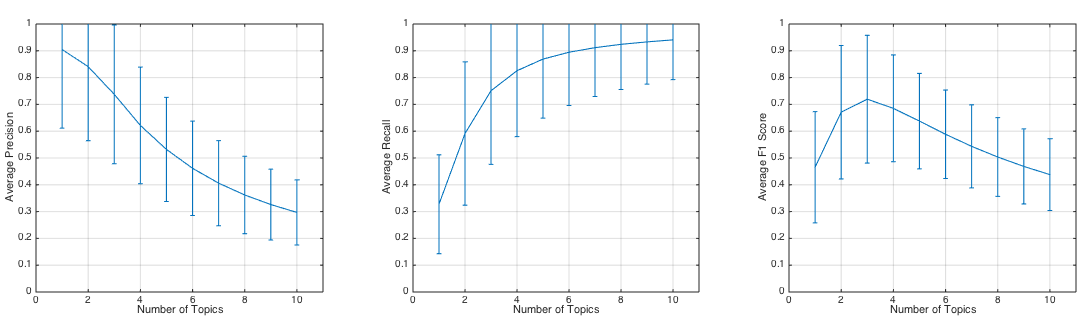
\includegraphics[width=1\textwidth]{nb.png}
    \caption{Performance of NB as the Number of Topics to Emit Increases}
    \label{fig:nb}
\end{figure}

\subsection{Logistic Regression}
\subsubsection*{Learning}
To train a LR classifier and to make predictions, a document $d$ is required to be transformed into a vector representation such that each entry of the vector indicates the term frequency of a specific word $w$.
This vector, together with its corresponding assigned set of topics, are used to train the classifier.
Note that during the vectorisation process, each word $w$ is uniquely assigned a fixed index based on its collection frequency such that the more frequent words get the smaller indices.
Therefore, each vector is actually of the length equal to the size of the vocabulary $V$.
In implementation, sparse vectors are used to reduce the memory footprint of the program.
Also, it is possible to specify the number of features to use for the SVM, and the features are selected based on their indices.

The LR classifier is trained using the Stochastic Gradient Descent (SGD) algorithm. 
However, some consideration must be taken since the number of positive classes and the number of negative classes are imbalanced in the training dataset.
The following equation shows the modified updating rule that is used to specifically address this problem.

\begin{equation}
    \label{eq:lr-update}
    \begin{split}
        \theta_{t, i+1} = \theta_{t, i} + \left\{
            \begin{array}{lr}
                (1 - logistic(d_i, \theta_{t, i})) d_i & : t\in topics(d_i) \\
                - logistic(d_i, \theta_{t, i}) d_i & : otherwise
            \end{array}
        \right.
    \end{split}
\end{equation}

\begin{equation}
    \label{eq:lr-logistic}
    \begin{split}
        logistic(d, \theta) = \cfrac{1}{1 + e^{-\theta^T d}}
    \end{split}
\end{equation}

\subsubsection*{Prediction}
The LR classifier implemented in this project predicts a variable number of topics for each document. It accepts the maximum number of topics to emit as an argument. 
In cases where the number of predicted topics exceeding that maximum number, only the top ranked maximum number of topics are emitted.

\begin{figure}[b]
\centering
    \centering
    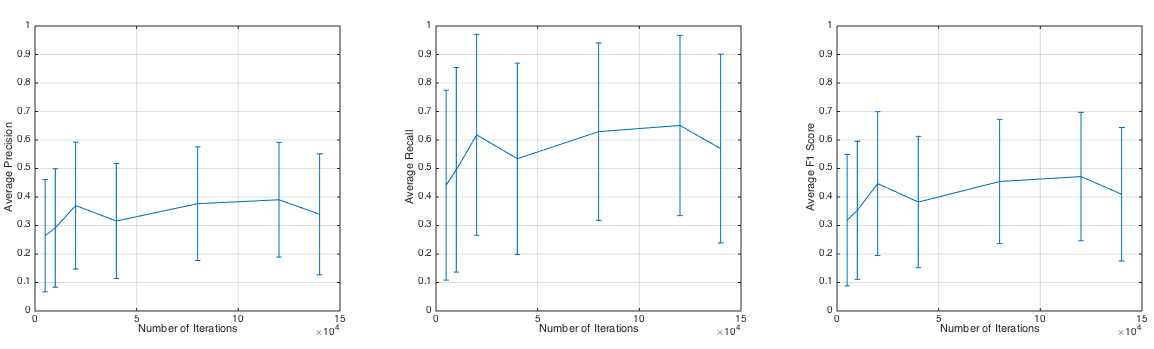
\includegraphics[width=1\textwidth]{lr-num-of-iterations.png}
    \caption{Learning Curve of the LR Classifier}
    \label{fig:lr-num-of-iterations}
\end{figure}

\begin{figure}
\centering
    \centering
    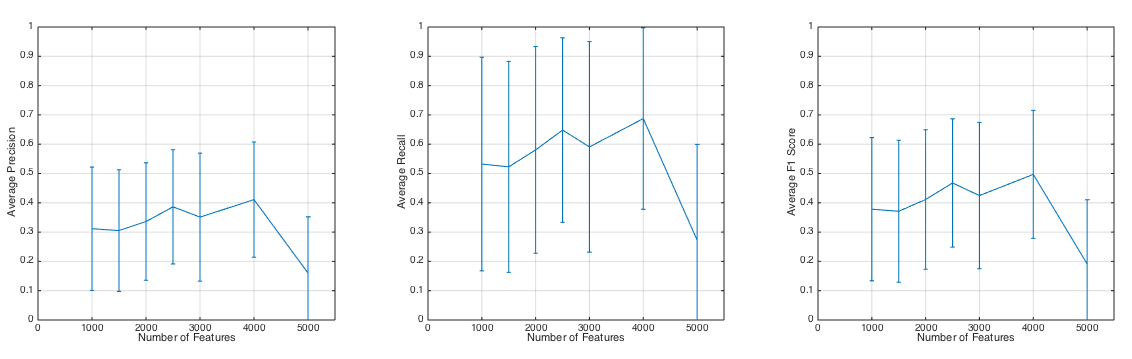
\includegraphics[width=1\textwidth]{lr-num-of-features.png}
    \caption{Performance of the LR Classifier as the Number of Features Increases}
    \label{fig:lr-num-of-features}
\end{figure}

\begin{figure}
\centering
    \centering
    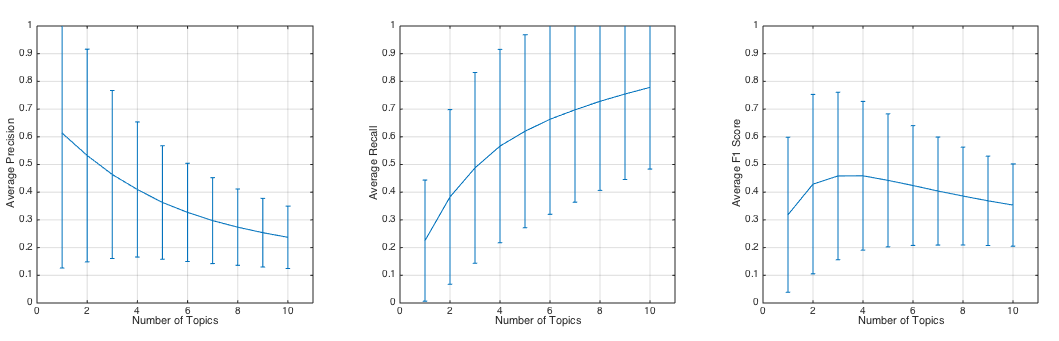
\includegraphics[width=1\textwidth]{lr-num-of-topics.png}
    \caption{Performance of LR Classifier as the Maximum Number of Features to Emit Increases}
    \label{fig:lr-num-of-topics}
\end{figure}

\subsubsection*{Performance}
Before evaluating the performance of this model, the effect of various parameters are studied.

\begin{itemize}
    \item{\textbf{Number of Iterations}: 
    Figure \ref{fig:lr-num-of-iterations} shows the learning curve of the LR classifier with \newline $num\_of\_features=2000$, and $max\_num\_of\_topics = 5$.
    }
    \item{\textbf{Number of Features}: 
    Figure \ref{fig:lr-num-of-features} shows the performance of the LR classifier with \newline$num\_of\_iterations=100000$, and $max\_num\_of\_topics = 10$.
    It can be seen that the prediction accuracy fluctuates as the size of the feature space changes.
    }
    \item{\textbf{Maximum Number of Topics}: 
    Figure \ref{fig:lr-num-of-topics} shows that the average F1 score of prediction increases as the maximum number of topics to emit increases to $3$.
    Then the F1 score decreases as the maximum number of topics to emit increases due to the degradation of the average precision.
    This experiment is conducted with $num\_of\_features=4000$, and $num\_of\_iterations = 120000$.
    }
\end{itemize}

With the above observations, the final prediction for submission uses  $num\_of\_features=4000$, $num\_of\_iterations = 100000$, and $max\_num\_of\_topics = 4$.
The corresponding average precision, average recall and average F1 score are $0.3676$, $0.5003$, and $0.4088$ respectively.

\subsection{Support Vector Machine}
\subsubsection*{Learning}
Similar to the LR classifier, the input to the SVM classifier also needs to be vectorised.
The vectorisation process is the same as the one used for the LR classifier.
It is also possible to specify the number of features to use for the SVM, and the underlying mechanism works the same as the LR classifier.

The SVM classifier is trained using the Pegasos algorithm \cite{pegasos}.
The reference at the end of the report provides a detailed description of the algorithm.
The following equations (\ref{eq:svm-update}) and (\ref{eq:svm-projection}) only show the update and the projection rule for the weight vector $\theta$ for each topic $t$.

\begin{equation}
    \label{eq:svm-y}
    \begin{split}
        y_{t, i} = \left\{
            \begin{array}{lr}
                1 & : document\ d_i\ is\ assigned\ to\ topic\ t \\
                -1 & : otherwise
            \end{array}
        \right.
    \end{split}
\end{equation}

\begin{equation}
    \label{eq:svm-update}
    \begin{split}
        \theta_{t, i+1} = \left\{
            \begin{array}{lr}
                (1 - \eta_i \lambda) \theta_{t, i} + \eta_i y_{t, i} d_i & : y_{t, i}\theta_t^T d_t < 0 \\
                (1 - \eta_i \lambda) \theta_{t, i} & : otherwise
            \end{array}
        \right.
    \end{split}
\end{equation}

\begin{equation}
    \label{eq:svm-projection}
    \begin{split}
        \theta_{t, i+1} = min\Bigg(1, \cfrac{\cfrac{1}{\sqrt{\lambda}}}{\left\lVert \theta_{t, i+1} \right\rVert} \Bigg)
    \end{split}
\end{equation}

\subsubsection*{Prediction}
The SVM classifier implemented in this project predicts a variable number of topics for each document.
It accepts the maximum number of topics to emit as an argument.
In cases where the number of predicted topics exceeding that maximum number, only the top ranked maximum number of topics are emitted.

\begin{figure}
\centering
    \centering
    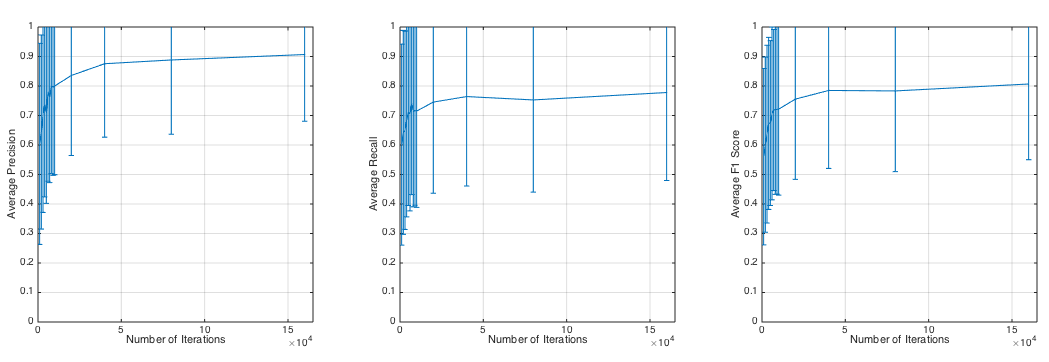
\includegraphics[width=1\textwidth]{svm-num-of-iterations.png}
    \caption{Learning Curve of the SVM Classifier}
    \label{fig:svm-num-of-iterations}
\end{figure}

\begin{figure}
\centering
    \centering
    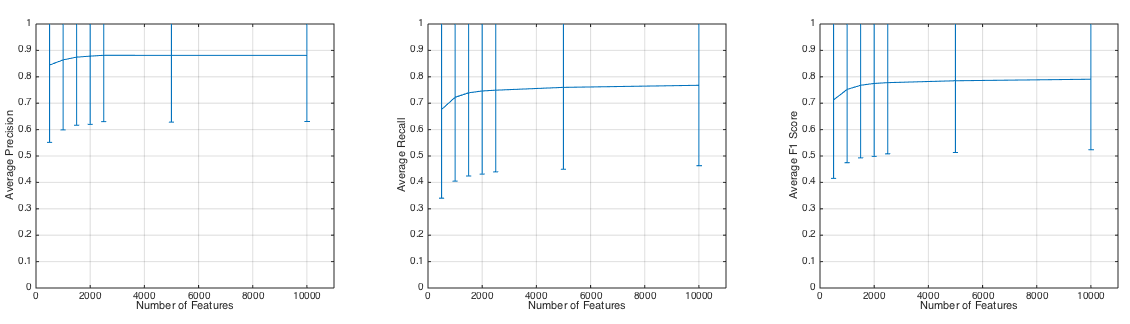
\includegraphics[width=1\textwidth]{svm-num-of-features.png}
    \caption{Performance of SVM as the Number of Features Increases}
    \label{fig:svm-num-of-features}
\end{figure}

\begin{figure}
\centering
    \centering
    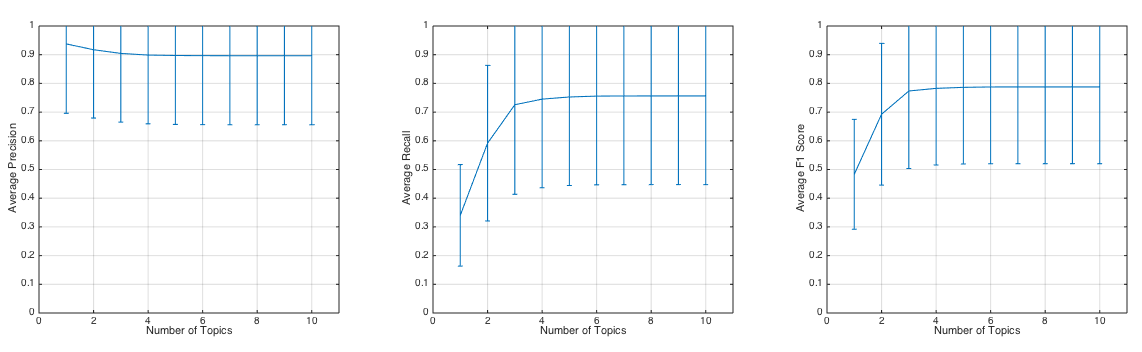
\includegraphics[width=1\textwidth]{svm-num-of-topics}
    \caption{Performance of SVM as the Maximum Number of Features to Emit Increases}
    \label{fig:svm-num-of-topics}
\end{figure}

\subsubsection*{Performance}
Before evaluating the performance of this model, the effect of various parameters are studied.

\begin{itemize}
    \item{\textbf{Number of Iterations}: 
    Figure \ref{fig:svm-num-of-iterations} shows the learning curve of the SVM with $\lambda=0.01$, $num\_of\_features=2000$, and $max\_num\_of\_topics = 10$.
    It can be seen that the prediction accuracy improves drastically during the first $20000$ iterations, and the improvement slows down afterwards.
    }
    \item{\textbf{$\lambda$}: 
    The choice of $\lambda$ also has impact on the performance of the SVM, which is summarised in Table \ref{table:svm_lambda}.
    }
    \item{\textbf{Number of Features}: 
    Figure \ref{fig:svm-num-of-features} shows the performance of the SVM with $\lambda=0.01$, \newline$num\_of\_iterations=15000$, and $max\_num\_of\_topics = 10$.
    It can be seen that the prediction accuracy is relatively insensitive to the size of the feature space after around $2000$.
    }
    \item{\textbf{Maximum Number of Topics}: 
    Figure \ref{fig:svm-num-of-topics} clearly indicates that the average F1 score of prediction increases as the maximum number of topics to emit increases to $4$.
    Then the F1 score stays almost unchanged, meaning that for most of the documents, the SVM only give $4$ positive feedbacks.
    This experiment is conducted with $\lambda=0.01$, $num\_of\_features=2000$, and $num\_of\_iterations = 15000$.
    }
\end{itemize}

With the above observations, the final prediction for submission uses  $\lambda=0.01$, $num\_of\_features=2000$, $num\_of\_iterations = 50000$, and $max\_num\_of\_topics = 10$.
The corresponding average precision, average recall and average F1 score are $0.9067$, $0.7779$, and $0.7778$ respectively.

\begin{table}
    \centering
    \makebox[500pt][c]{
        \begin{minipage}{0.7\textwidth}
            \centering
            \caption{Performance of SVM as $\lambda$ Increases}
            \begin{tabular}{ c | c | c }
                \hline
                $\lambda$ & Mean F1 Score & Std F1 Score \\ \hline
                $0.0001$ & $0.6107$ &  $0.2889$ \\ \hline
                $0.001$ & $0.7024$ &  $0.2774$ \\ \hline
                $0.01$ & $0.7483$ &  $0.2713$ \\ \hline
                $0.1$ & $0.6696$ &  $0.3100$ \\ \hline
                $1$ & $0.4682$ & $0.3112$\\ \hline
            \end{tabular}    
            \label{table:svm_lambda}
        \end{minipage}
    }
\end{table}

\subsection{Summary}
This sections summarises the performance of the three models discussed before. The details are listed in Table \ref{table:summary}.


\begin{table}
    \centering
    \makebox[500pt][c]{
        \begin{minipage}{1\textwidth}
            \centering
            \caption{Summary of Three Text Categorisation Models}
            \begin{tabular}{ c | c | c | c }
                \hline
                Model & Mean Precision & Mean Recall & Mean F1 \\ \hline
                NB & $0.7374$ & $0.7510$ & $0.7194$ \\ \hline
                LR & $0.3676$ & $0.5003$ & $0.4088$ \\ \hline
                SVM & $0.9067$ & $0.7779$ & $0.7778$ \\ \hline
            \end{tabular}    
            \label{table:summary}
        \end{minipage}
    }
\end{table}


\section{How to Run the Program}

\subsection{Dependencies}
To compile and run the source code, the following dependencies need to be installed:
\begin{itemize}
    \item{Breeze v0.10\footnote{https://github.com/scalanlp/breeze}}
    \item{Processors v3.3\footnote{https://github.com/sistanlp/processors}}
    \item{Stanford CoreNLP models v3.3.1\footnote{http://nlp.stanford.edu/software/corenlp.shtml}}
\end{itemize}

\subsection{Command Line Arguments}
The program expects the following command line arguments in the ordered specified:
\begin{itemize}
    \item{Model to use for learning: "nb", "lr", or "svm"}
    \item{Path to the training dataset directory}
    \item{Path to the validation dataset directory}
    \item{Path to the testing dataset directory}
    \item{Path to the directory to which submission files are written}
\end{itemize}
Note that for the dataset, the top level zip file needs to be unzipped first, e.g. the train.zip file.

\begin{thebibliography}{9}

\bibitem{pegasos}
    Shalev-Shwartz, Shai and Singer, Yoram and Srebro, Nathan
    \emph{Pegasos: Primal Estimated sub-GrAdient SOlver for SVM}.
    Proceedings of the 24th International Conference on Machine Learning.
    ICML '07.
    2007.
\end{thebibliography}

\end{document}